\documentclass[12pt,a4paper]{report}

\PassOptionsToPackage{hyphens}{url}

\usepackage[utf8]{inputenc}
\usepackage[T5]{fontenc}
\usepackage[vietnamese]{babel}
\usepackage{amsmath, amssymb, amsthm}
\usepackage{bm}
\usepackage{graphicx}
\usepackage{float}
\usepackage{subcaption}
\usepackage{booktabs}
\usepackage{array}
\usepackage{longtable}
\usepackage{multirow}
\usepackage[table]{xcolor}
\usepackage{hyperref}
\usepackage{url}
\usepackage[ruled,vlined]{algorithm2e}
\usepackage{listings}
\usepackage{geometry}
\usepackage{fancyhdr}
\usepackage{titlesec}
\usepackage{enumitem}
\usepackage{caption}
\usepackage{tcolorbox}
\usepackage{mathtools}
\usepackage{setspace}
\usepackage{tikz}
\usepackage{tabularx}
\usetikzlibrary{arrows.meta, calc, positioning, shapes.geometric, shapes.misc, decorations.pathreplacing, matrix,shapes.geometric, arrows.meta, positioning, fit, backgrounds, calc}

\geometry{a4paper, top=2.5cm, bottom=2.5cm, left=3cm, right=2.5cm, headheight=14.5pt}
\onehalfspacing
\setlength{\parindent}{1.25cm}
\setlength{\parskip}{0pt}
\setlength{\emergencystretch}{3em}
\hfuzz=140pt
\hbadness=10000

\definecolor{myblue}{RGB}{31, 73, 125}
\definecolor{hcmusblue}{RGB}{0, 82, 155}
\definecolor{mygray}{RGB}{245, 245, 245}
\definecolor{mygreen}{RGB}{0, 128, 0}
\definecolor{myred}{RGB}{180, 0, 0}
\definecolor{codebg}{RGB}{248, 248, 248}
\definecolor{tableheadbg}{RGB}{230, 240, 250}

\hypersetup{colorlinks=true, linkcolor=myblue, citecolor=myblue, urlcolor=myblue}

\pagestyle{fancy}
\fancyhf{}
\fancyhead[L]{\small CSC14005 -- Học thống kê}
\fancyhead[R]{\small ViMedAQA -- Hỏi đáp y khoa}
\fancyfoot[C]{\thepage}
\renewcommand{\headrulewidth}{0.4pt}

\newtheorem{theorem}{Định lý}[chapter]
\newtheorem{definition}{Định nghĩa}[chapter]
\newtheorem{proposition}{Mệnh đề}[chapter]
\newtheorem{remark}{Nhận xét}[chapter]

\tcbuselibrary{skins, breakable}
\newtcolorbox{notebox}{colback=mygray, colframe=myblue, fonttitle=\bfseries, title=Lưu ý, breakable}
\newtcolorbox{resultbox}{colback=green!5, colframe=mygreen, fonttitle=\bfseries, title=Kết quả, breakable}
\newtcolorbox{expandbox}{colback=yellow!12, colframe=orange!80!black, fonttitle=\bfseries, title={[Mở rộng]}, breakable}

\lstset{backgroundcolor=\color{codebg}, basicstyle=\ttfamily\footnotesize, breaklines=true, frame=single, language=Python, keywordstyle=\color{myblue}\bfseries, commentstyle=\color{mygreen}, stringstyle=\color{myred}, numbers=left, numberstyle=\tiny\color{gray}, xleftmargin=1.5em}

\titleformat{\chapter}[display]
  {\normalfont\huge\bfseries\color{myblue}\centering}
  {Chương \thechapter}
  {0.5em}
  {\Huge}
\titlespacing*{\chapter}{0pt}{-10pt}{28pt}
\titleformat{\section}{\Large\bfseries\color{myblue}}{\thesection}{1em}{}[\titlerule]
\titleformat{\subsection}{\large\bfseries\color{myblue!80!black}}{\thesubsection}{1em}{}
\titleformat{\subsubsection}{\normalsize\bfseries\color{myblue!70!black}}{\thesubsubsection}{1em}{}
\setcounter{secnumdepth}{3}
\setcounter{tocdepth}{3}

\renewcommand{\contentsname}{Mục lục}
\renewcommand{\listfigurename}{Danh sách các hình}
\renewcommand{\listtablename}{Danh sách các bảng}
\renewcommand{\bibname}{Tài liệu tham khảo}

\begin{document}
\pagenumbering{gobble}
\hypersetup{pageanchor=false}
% BÌA THEO MẪU BÁO CÁO
\begin{titlepage}
  \thispagestyle{empty}
  \begin{tikzpicture}[remember picture, overlay]
    \draw[line width=3pt, color=myblue]
      ($(current page.south west) + (2cm, 2cm)$)
      rectangle
      ($(current page.north east) + (-2cm, -2cm)$);
    \draw[line width=1pt, color=myblue]
      ($(current page.south west) + (2.15cm, 2.15cm)$)
      rectangle
      ($(current page.north east) + (-2.15cm, -2.15cm)$);
  \end{tikzpicture}

  \centering
  \vspace*{0.8cm}

  {\large\textbf{TRƯỜNG ĐẠI HỌC KHOA HỌC TỰ NHIÊN}}\\[0.35em]
  {\large\textbf{KHOA CÔNG NGHỆ THÔNG TIN}}

  \vspace{1.2cm}
  {\large\bfseries NGUYỄN KIM QUỐC -- NGUYỄN TIẾN THÀNH -- PHẠM MINH THÔNG}

  \vspace{1.6cm}
  {\Huge\bfseries\color{hcmusblue} HỎI ĐÁP Y KHOA TIẾNG VIỆT}\\[0.5em]
  {\LARGE\bfseries\color{myblue} TRÊN BỘ DỮ LIỆU ViMedAQA}\\[1.2em]
  \rule{12cm}{1.3pt}\\[1.2em]
  {\Large\bfseries ĐỒ ÁN}\\[0.35em]
  {\large\bfseries HỌC THỐNG KÊ}

  \vspace{1cm}
  {\large CỬ NHÂN CÔNG NGHỆ THÔNG TIN}\\[0.35em]
  {\large CHƯƠNG TRÌNH CHÍNH QUY CHUẨN}

  \vfill

  \begin{tabular}{ll}
    \textbf{Giảng viên hướng dẫn:} & Th.S Lê Long Quốc \\[0.35em]
    \textbf{Môn học:}              & Học thống kê (CSC14005) \\[0.35em]
    \textbf{Học kỳ:}               & Học kỳ 2 -- 2025/2026 \\
  \end{tabular}

  \vspace{1cm}
  {\small TP. Hồ Chí Minh, tháng 05/2026}
\end{titlepage}
\clearpage

\begin{titlepage}
  \thispagestyle{empty}
  \centering
  \vspace*{0.8cm}
  {\large\textbf{TRƯỜNG ĐẠI HỌC KHOA HỌC TỰ NHIÊN - ĐHQG TPHCM}}\\[0.35em]
  {\large\textbf{KHOA CÔNG NGHỆ THÔNG TIN}}

  \vspace{1.2cm}
  \begin{tabular}{rl}
    Nguyễn Kim Quốc       & 23120347 \\
    Nguyễn Tiến Thành     & 23120358\\
    Phạm Minh Thông       & 23120364 \\
  \end{tabular}

  \vspace{1.8cm}
  {\Huge\bfseries\color{hcmusblue} HỎI ĐÁP Y KHOA TIẾNG VIỆT}\\[0.5em]
  {\LARGE\bfseries\color{myblue} TRÊN BỘ DỮ LIỆU ViMedAQA}\\[1.2em]
  \rule{12cm}{1.3pt}\\[1.2em]
  {\Large\bfseries ĐỒ ÁN -- HỌC THỐNG KÊ}\\[0.7em]

  \vfill
  {\large\bfseries GIẢNG VIÊN HƯỚNG DẪN}\\[0.5em]
  {\large Th.S Lê Long Quốc}

  \vspace{1.2cm}
  {\small TP. Hồ Chí Minh, tháng 05/2026}
\end{titlepage}
\clearpage
\hypersetup{pageanchor=true}

\pagenumbering{roman}
\chapter*{Lời cam đoan}
\addcontentsline{toc}{chapter}{Lời cam đoan}
Chúng tôi xin cam đoan báo cáo này là công trình học tập và nghiên cứu của nhóm dưới sự hướng dẫn của giảng viên phụ trách môn học. Các nội dung tham khảo đều được trích dẫn và liệt kê trong phần tài liệu tham khảo.

\vspace{2cm}
\begin{flushright}
\begin{tabular}{c}
TP. Hồ Chí Minh, \today \\
\textbf{Đại diện nhóm thực hiện} \\
\vspace{1.8cm} \\
Nguyễn Kim Quốc
\end{tabular}
\end{flushright}
\clearpage

\chapter*{Lời cảm ơn}
\addcontentsline{toc}{chapter}{Lời cảm ơn}
Nhóm xin chân thành cảm ơn Th.S Lê Long Quốc đã hướng dẫn, góp ý và hỗ trợ trong quá trình thực hiện đồ án Học thống kê. Nhóm cũng cảm ơn Khoa Công nghệ Thông tin, Trường Đại học Khoa học Tự nhiên, ĐHQG-HCM đã tạo điều kiện học tập và nghiên cứu thuận lợi.
\clearpage
\tableofcontents
\clearpage
\listoffigures
\clearpage
\listoftables
\clearpage
\chapter*{Tóm tắt}
\addcontentsline{toc}{chapter}{Tóm tắt}
Báo cáo này trình bày quy trình nghiên cứu, xây dựng và đánh giá thực nghiệm hệ thống hỏi đáp trừu tượng tiếng Việt trong miền y khoa dựa trên bộ dữ liệu ViMedAQA. Khác với nhiệm vụ hỏi đáp trích xuất truyền thống, hỏi đáp trừu tượng y khoa đòi hỏi mô hình phải hiểu sâu sắc ngữ cảnh và sinh câu trả lời tự nhiên, trôi chảy và chính xác về mặt y khoa. Chúng tôi thực hiện nghiên cứu so sánh hai kiến trúc sinh chuỗi chuyên biệt cho tiếng Việt là ViT5-base và BARTpho-word bằng cách tinh chỉnh (fine-tuning) trên tập dữ liệu gồm 23.553 mẫu. Đồng thời, mô hình ngôn ngữ lớn Llama-3.3-70B-versatile được tích hợp làm đường cơ sở (baseline) dưới dạng zero-shot thông qua Groq API để làm hệ quy chiếu đánh giá. Kết quả kiểm thử định lượng cho thấy cả hai mô hình tinh chỉnh đều đạt hiệu năng vượt trội. Cụ thể, ViT5-base đạt điểm ROUGE-L là 66,80\%, BLEU-4 là 50,05\% và BERTScore F1 là 87,52\%, trong khi BARTpho-word đạt ROUGE-L là 66,81\% và BERTScore F1 là 82,30\%. Đáng chú ý, baseline Llama-3.3 zero-shot thể hiện khả năng vượt trội với BERTScore F1 đạt 87,57\% nhờ tri thức nền tảng khổng lồ. Báo cáo cũng phân tích sâu sắc các nhóm lỗi sinh văn bản thực tế (lặp từ, ảo tưởng thông tin y khoa, độ lệch chiều dài) và nghiên cứu sự ảnh hưởng của chiến lược giải mã (beam search giúp cải thiện 0,6\% điểm ROUGE so với greedy decoding). Cuối cùng, một ứng dụng minh họa Gradio tích hợp cơ chế truy xuất thông tin BM25 (RAG) đã được triển khai và công bố công khai. Kết quả nghiên cứu đóng góp một pipeline hoàn chỉnh, có khả năng tái lập cao cho các ứng dụng y tế thông minh bằng tiếng Việt.
\clearpage

\clearpage
\pagenumbering{arabic}
\chapter{Giới thiệu}
\section{Bối cảnh và động lực}
Trong những năm gần đây, sự phát triển vượt bậc của các mô hình ngôn ngữ lớn dựa trên kiến trúc Transformer \cite{vaswani2017attention} đã mở ra nhiều hướng nghiên cứu mới trong lĩnh vực xử lý ngôn ngữ tự nhiên (NLP), đặc biệt là trong miền y khoa. Các hệ thống hỏi đáp y khoa tự động đóng vai trò vô cùng quan trọng trong việc hỗ trợ các chuyên gia y tế tra cứu thông tin nhanh chóng, đồng thời giúp bệnh nhân tiếp cận các kiến thức chăm sóc sức khỏe chính thống, đáng tin cậy. 

Tuy nhiên, việc xây dựng một hệ thống hỏi đáp y khoa hiệu quả đối với tiếng Việt vẫn đang đối mặt với nhiều thách thức lớn do tính chất khan hiếm tài nguyên ngôn ngữ và sự phức tạp của thuật ngữ chuyên ngành. Phần lớn các nghiên cứu hỏi đáp trước đây tại Việt Nam tập trung vào bài toán hỏi đáp trích xuất (Extractive Question Answering), trong đó câu trả lời bắt buộc phải là một đoạn văn bản (span) nằm nguyên văn trong ngữ cảnh cung cấp sẵn. Phương pháp này bộc lộ hạn chế lớn khi áp dụng vào thực tế y khoa, nơi người bệnh thường cần những câu trả lời được tổng hợp, diễn giải một cách ngắn gọn, dễ hiểu và tự nhiên thay vì một đoạn văn bản kỹ thuật phức tạp được trích xuất cứng nhắc.

Nhằm giải quyết hạn chế đó, bộ dữ liệu ViMedAQA \cite{tran2024vimedaqa} đã được giới thiệu tại Hội nghị ACL 2024 như một bộ dữ liệu tiên phong cho bài toán hỏi đáp y khoa trừu tượng (Abstractive Question Answering) bằng tiếng Việt. Trong bài toán hỏi đáp trừu tượng, mô hình phải tự sinh ra (generate) câu trả lời bằng cách diễn giải, Paraphrase và tổng hợp thông tin từ ngữ cảnh y khoa được cung cấp. Do đó, việc áp dụng các kiến trúc sinh chuỗi từ văn bản sang văn bản (Sequence-to-Sequence) là cực kỳ cấp thiết để mô hình hóa trọn vẹn bản chất của bài toán này.

\section{Mục tiêu đề tài}
Đề tài nghiên cứu này hướng đến việc thiết lập, huấn luyện và đánh giá một quy trình thực nghiệm (pipeline) toàn diện cho bài toán hỏi đáp y khoa trừu tượng tiếng Việt trên bộ dữ liệu ViMedAQA \cite{tran2024vimedaqa}. Cụ thể, các mục tiêu chi tiết bao gồm:
\begin{itemize}
  \item Khảo sát sâu sắc và chuẩn hóa dữ liệu y khoa từ bộ dữ liệu ViMedAQA, xây dựng chiến lược chia tập huấn luyện (Train), kiểm định (Validation), và kiểm thử (Test) một cách đồng nhất, phân tầng (stratified) theo chủ đề.
  \item Tinh chỉnh (fine-tuning) hai mô hình sinh ngôn ngữ chuyên biệt cho tiếng Việt là ViT5-base và BARTpho-word trên tập dữ liệu y khoa, tối ưu hóa các siêu tham số huấn luyện để đạt được hiệu năng cao nhất trong điều kiện tài nguyên tính toán giới hạn.
  \item Xây dựng một baseline zero-shot sử dụng mô hình ngôn ngữ lớn Llama-3.3-70B-versatile thông qua Groq API để tạo điểm tham chiếu thực tế cho việc đánh giá sức mạnh của phương pháp tinh chỉnh chuyên biệt so với mô hình tổng quát.
  \item Thực hiện phân tích định lượng toàn diện bằng các độ đo tự động chuẩn quốc tế (ROUGE-1/2/L, BLEU-4, BERTScore F1) kết hợp với phân tích định tính các nhóm lỗi sinh văn bản thực tế để chỉ ra các thách thức khoa học còn tồn tại.
  \item Phát triển ứng dụng Web Gradio tích hợp cơ chế Retrieval-Augmented Generation (RAG) và triển khai trên môi trường đám mây công khai để chứng minh tính thực tiễn của đề tài.
\end{itemize}

\section{Đóng góp chính}
Các đóng góp chính của đề tài nghiên cứu này bao gồm:
\begin{itemize}
  \item Đề xuất một khung thực nghiệm chuẩn hóa, có tính nhất quán cao cho bài toán hỏi đáp trừu tượng y khoa tiếng Việt, giải quyết bài toán OOM (Out Of Memory) trên phần cứng giới hạn (GPU T4) bằng các kỹ thuật tích lũy gradient (gradient accumulation) và độ dài cắt tỉa phù hợp.
  \item Cung cấp bảng so sánh thực nghiệm chi tiết và công bằng giữa hai họ mô hình Sequence-to-Sequence phổ biến (T5 vs BART) được tối ưu riêng cho tiếng Việt trên cùng một tập dữ liệu y khoa chuyên biệt.
  \item Minh chứng thực nghiệm rằng mô hình nhỏ được tinh chỉnh chuyên biệt (ViT5-base, ~270M tham số) hoàn toàn có khả năng cạnh tranh sòng phẳng hoặc thậm chí vượt trội hơn mô hình ngôn ngữ lớn tổng quát (Llama-3.3-70B) trên một số độ đo trùng khớp chuỗi (BLEU-4).
  \item Thiết lập một quy trình phân tích lỗi hệ thống, phân loại cụ thể các hiện tượng ảo tưởng thông tin (factual hallucination) và lặp từ trong sinh câu y khoa, đặt nền móng cho các nghiên cứu cải thiện độ an toàn y tế của LLM.
  \item Triển khai thành công hệ thống demo RAG thực tế chạy trên HuggingFace Spaces, cho phép người dùng hỏi đáp y khoa mà không cần tự cung cấp ngữ cảnh đầu vào nhờ cơ chế truy xuất tự động BM25 trên kho tri thức y học.
\end{itemize}
\chapter{Cơ sở lý thuyết và công trình liên quan}
\section{Bài toán hỏi đáp trừu tượng y khoa}
Cho câu hỏi y tế $q$, ngữ cảnh y khoa liên quan $c$ và câu trả lời y tế tham chiếu $a$. Trong bài toán hỏi đáp trừu tượng, mục tiêu của mô hình là học phân phối xác suất có điều kiện trên chuỗi các token của câu trả lời $a = (a_1, a_2, \dots, a_T)$:
\begin{equation}
  p(a \mid q, c) = \prod_{t=1}^{T} p(a_t \mid a_{<t}, q, c),
\end{equation}
trong đó $a_{<t} = (a_1, \dots, a_{t-1})$ là các token đã được sinh ra trước thời điểm $t$. 

Khác hoàn toàn với bài toán trích xuất (chỉ tìm hai chỉ số vị trí bắt đầu và kết thúc của câu trả lời trong ngữ cảnh), mô hình trừu tượng phải tự sinh chuỗi (sequence generation) bằng cách chuyển dịch không gian ngữ nghĩa từ đầu vào $x = [q; c]$ sang đầu ra $y = a$. Do đó, mô hình cần học cách mã hóa ngữ nghĩa đầu vào và giải mã tuần tự để tạo ra câu trả lời tự nhiên.

\section{Kiến trúc Transformer và Cơ chế Attention}
Kiến trúc Transformer \cite{vaswani2017attention} dựa trên cơ chế tự chú ý (self-attention) đóng vai trò nền tảng cho việc biểu diễn thông tin ngữ nghĩa dài. Cơ chế attention được định nghĩa thông qua ma trận truy vấn $Q$, khóa $K$ và giá trị $V$:
\begin{equation}
  \operatorname{Attention}(Q, K, V) = \operatorname{softmax}\left(\frac{QK^\top}{\sqrt{d_k}}\right)V,
\end{equation}
trong đó $d_k$ là chiều vectơ của khóa (dimension key) đóng vai trò như một thừa số tỷ lệ (scaling factor) nhằm tránh hiện tượng gradient bị triệt tiêu khi tích vô hướng có giá trị quá lớn.

Để mô hình hóa nhiều mối quan hệ ngữ nghĩa ở các không gian biểu diễn khác nhau, Transformer mở rộng thành cơ chế chú ý nhiều đầu (Multi-Head Attention - MHA):
\begin{equation}
  \operatorname{MultiHead}(Q, K, V) = \operatorname{Concat}(\operatorname{head}_1, \dots, \operatorname{head}_h)W^O,
\end{equation}
\begin{equation}
  \text{trong đó: } \operatorname{head}_i = \operatorname{Attention}(QW_i^Q, KW_i^K, VW_i^V),
\end{equation}
và các ma trận $W_i^Q \in \mathbb{R}^{d_{model} \times d_k}$, $W_i^K \in \mathbb{R}^{d_{model} \times d_k}$, $W_i^V \in \mathbb{R}^{d_{model} \times d_v}$, $W^O \in \mathbb{R}^{h d_v \times d_{model}}$ là các tham số chiếu học được trong quá trình huấn luyện.

\section{Kiến trúc sinh chuỗi Sequence-to-Sequence}
Mô hình Sequence-to-Sequence (Seq2Seq) trong đề tài bao gồm một bộ mã hóa (Encoder) và một bộ giải mã (Decoder). Bộ mã hóa nhận đầu vào $x$ và sinh ra biểu diễn ẩn liên tục $z = (z_1, \dots, z_n)$. Bộ giải mã nhận $z$ và sinh tuần tự từng token đầu ra $y_t$ dựa trên các token đã sinh $y_{<t}$ và biểu diễn $z$ thông qua cơ chế chú ý chéo (Cross-Attention).

\subsection{ViT5-base}
ViT5 \cite{phan2022vit5} là mô hình ngôn ngữ dựa trên kiến trúc T5 (Text-to-Text Transfer Transformer) tiền huấn luyện chuyên biệt cho tiếng Việt. ViT5 sử dụng kiến trúc Encoder-Decoder tiêu chuẩn với các khối chuẩn hóa Layer Normalization cải tiến (như RMSNorm) và mã hóa vị trí tương đối. ViT5 được tiền huấn luyện trên lượng dữ liệu tiếng Việt khổng lồ với hai tác vụ chính: điền chỗ trống (span corruption) và sinh văn bản tự do. ViT5-base với khoảng 270 triệu tham số được chứng minh đạt hiệu năng SOTA trên nhiều tác vụ sinh chuỗi tiếng Việt như tóm tắt văn bản và dịch máy.

\subsection{BARTpho-word}
BARTpho \cite{tran2021bartpho} là mô hình Sequence-to-Sequence đầu tiên được tiền huấn luyện cho tiếng Việt dựa trên kiến trúc BART (Bidirectional and Auto-Regressive Transformers). BARTpho kế thừa khả năng mã hóa hai chiều của BERT và khả năng tự hồi quy giải mã của GPT. Phiên bản BARTpho-word (khoảng 396 triệu tham số) được tiền huấn luyện trên dữ liệu tiếng Việt đã được tách từ (word-segmentation). Việc sử dụng tokenizer cấp từ giúp BARTpho biểu diễn tốt các từ ghép tiếng Việt và giảm thiểu chiều dài chuỗi đầu vào, tối ưu hóa khả năng hiểu ngữ nghĩa y khoa phức tạp.

\subsection{Đường cơ sở Zero-shot và Mô hình Đa ngôn ngữ}
Đường cơ sở Llama-3.3-70B-versatile đại diện cho dòng mô hình ngôn ngữ lớn (LLM) chỉ chứa bộ giải mã (Decoder-only) tiên tiến nhất hiện nay, được chạy dưới dạng zero-shot để kiểm chứng năng lực giải quyết bài toán y khoa chuyên sâu khi không có bất kỳ bước tinh chỉnh tham số nào. Ngoài ra, mô hình mT5-base \cite{xue2021mt5} (kiến trúc T5 đa ngôn ngữ, ~580M tham số) được đưa vào nghiên cứu mở rộng nhằm làm sáng tỏ lợi ích của tiền huấn luyện chuyên biệt đơn ngữ (ViT5) so với tiền huấn luyện đa ngôn ngữ diện rộng.
\chapter{Dữ liệu ViMedAQA}
\section{Mô tả bộ dữ liệu}
ViMedAQA \cite{tran2024vimedaqa} là bộ dữ liệu hỏi đáp trừu tượng tiếng Việt trong miền y khoa chất lượng cao. Khác biệt với các bộ dữ liệu hỏi đáp trích xuất (Extractive Question Answering) thông thường khi câu trả lời chỉ là một phân đoạn văn bản (span) được cắt trực tiếp từ ngữ cảnh, ViMedAQA tập trung vào bài toán hỏi đáp trừu tượng (Abstractive Question Answering). Trong miền y khoa, câu trả lời trừu tượng mang lại giá trị thực tiễn rất cao vì bệnh nhân và chuyên gia y tế thường yêu cầu những phản hồi được tổng hợp, diễn giải một cách tự nhiên và mạch lạc từ nhiều nguồn thông tin khác nhau. 

Mỗi mẫu dữ liệu trong ViMedAQA bao gồm bốn trường thông tin cốt lõi:
\begin{itemize}
    \item \textbf{Câu hỏi (Question):} Các truy vấn y tế bằng tiếng Việt tự nhiên do người dùng đặt ra, xoay quanh các triệu chứng, phương pháp điều trị, dược phẩm, hoặc kiến thức y học phổ thông.
    \item \textbf{Ngữ cảnh (Context):} Phân đoạn kiến thức y khoa đáng tin cậy được trích xuất từ các tài liệu chuyên ngành, bài báo y học uy tín hoặc hướng dẫn lâm sàng chính thức. Ngữ cảnh này đóng vai trò là nguồn tri thức nền tảng để trả lời câu hỏi.
    \item \textbf{Câu trả lời (Answer):} Câu trả lời chuẩn mực do các chuyên gia y tế hoặc người biên soạn có chuyên môn xây dựng. Câu trả lời này được tổng hợp và diễn đạt lại từ ngữ cảnh một cách ngắn gọn, súc tích và dễ hiểu đối với người bệnh.
    \item \textbf{Chủ đề (Topic):} Nhãn số phân loại chủ đề y khoa tương ứng (gồm 4 chủ đề từ 0 đến 3), giúp mô hình hóa phân phối của các chuyên khoa khác nhau.
\end{itemize}

\section{Định dạng dữ liệu đầu vào cho Seq2Seq}
Để huấn luyện và đánh giá các mô hình Sequence-to-Sequence (Seq2Seq) như ViT5 \cite{phan2022vit5} và BARTpho \cite{tran2021bartpho}, dữ liệu cần được chuẩn hóa về một định dạng chuỗi thống nhất. Định dạng này giúp mô hình phân biệt rõ ràng giữa câu hỏi cần trả lời và ngữ cảnh tri thức đi kèm. Cụ thể, định dạng đầu vào và đầu ra được thiết lập như sau:
\begin{tcolorbox}[colback=codebg, colframe=myblue, title={Định dạng đầu vào/đầu ra thống nhất cho các mô hình Seq2Seq}]
\small\ttfamily
INPUT : question: \{question\} context: \{context\}\par
OUTPUT: \{answer\}
\end{tcolorbox}


\section{Khảo sát dữ liệu thực tế và phân tích EDA}
Quy trình khám phá dữ liệu (Exploratory Data Analysis - EDA) được thực hiện kỹ lưỡng nhằm đánh giá chất lượng phân phối của bộ dữ liệu trước khi huấn luyện. Chúng tôi tiến hành kiểm tra số lượng mẫu, phân phối chủ đề, thống kê độ dài văn bản và đặc biệt là độ trùng khớp từ vựng (vocabulary overlap) giữa câu trả lời và ngữ cảnh. Kết quả thống kê chi tiết của bộ dữ liệu ViMedAQA được tổng hợp tại Bảng~\ref{tab:dataset_stats}.

\begin{table}[H]
\centering
\caption{Thống kê mô tả chi tiết bộ dữ liệu ViMedAQA thực tế}
\label{tab:dataset_stats}
\resizebox{\textwidth}{!}{%
\begin{tabular}{lr}
\toprule
\textbf{Chỉ số thống kê} & \textbf{Giá trị thực nghiệm} \\
\midrule
Tổng số mẫu dữ liệu sạch & 23.553 \\
Kích thước tập huấn luyện (Train split - 80\%) & 18.842 \\
Kích thước tập kiểm định (Validation split - 10\%) & 2.355 \\
Kích thước tập kiểm thử (Test split - 10\%) & 2.356 \\
Số lượng chủ đề y khoa độc lập & 4 \\
Độ trùng khớp từ vựng trung bình (Extractive Overlap) & 82,25\% \\
Độ dài ngữ cảnh trung bình (ViT5 Tokenizer) & 115,36 tokens (Max: 1517) \\
Độ dài ngữ cảnh trung bình (BARTpho Tokenizer) & 121,96 tokens (Max: 1523) \\
\bottomrule
\end{tabular}%
}
\end{table}

Chỉ số độ trùng khớp từ vựng trung bình đạt \textbf{82,25\%} phản ánh đặc tính \textit{semi-abstractive} (bán trừu tượng) của bộ dữ liệu. Mặc dù câu trả lời giữ lại một lượng lớn thuật ngữ chuyên ngành và thực thể y học quan trọng từ ngữ cảnh để đảm bảo tính chính xác khoa học, cấu trúc câu vẫn được tái cấu trúc và viết lại một cách tự nhiên. Thêm vào đó, sự khác biệt về độ dài token trung bình giữa hai bộ mã hóa (115,36 của ViT5 và 121,96 của BARTpho) xuất phát từ cách tiếp cận phân tách từ ngữ của các tokenizer: ViT5 sử dụng SentencePiece mức âm tiết, trong khi BARTpho sử dụng tokenizer cấp từ (word-level) dựa trên thư viện PyVi làm giàu thông tin ngữ nghĩa nhưng tạo ra các chuỗi dài hơn khi gặp từ chuyên ngành ghép nối bằng dấu gạch dưới (\texttt{\_}).

Để trực quan hóa sự phân phối độ dài của các trường dữ liệu quan trọng, chúng tôi vẽ biểu đồ phân phối độ dài của câu hỏi, ngữ cảnh và câu trả lời trong tập dữ liệu (xem Hình~\ref{fig:length_dist}).

\begin{figure}[H]
    \centering
    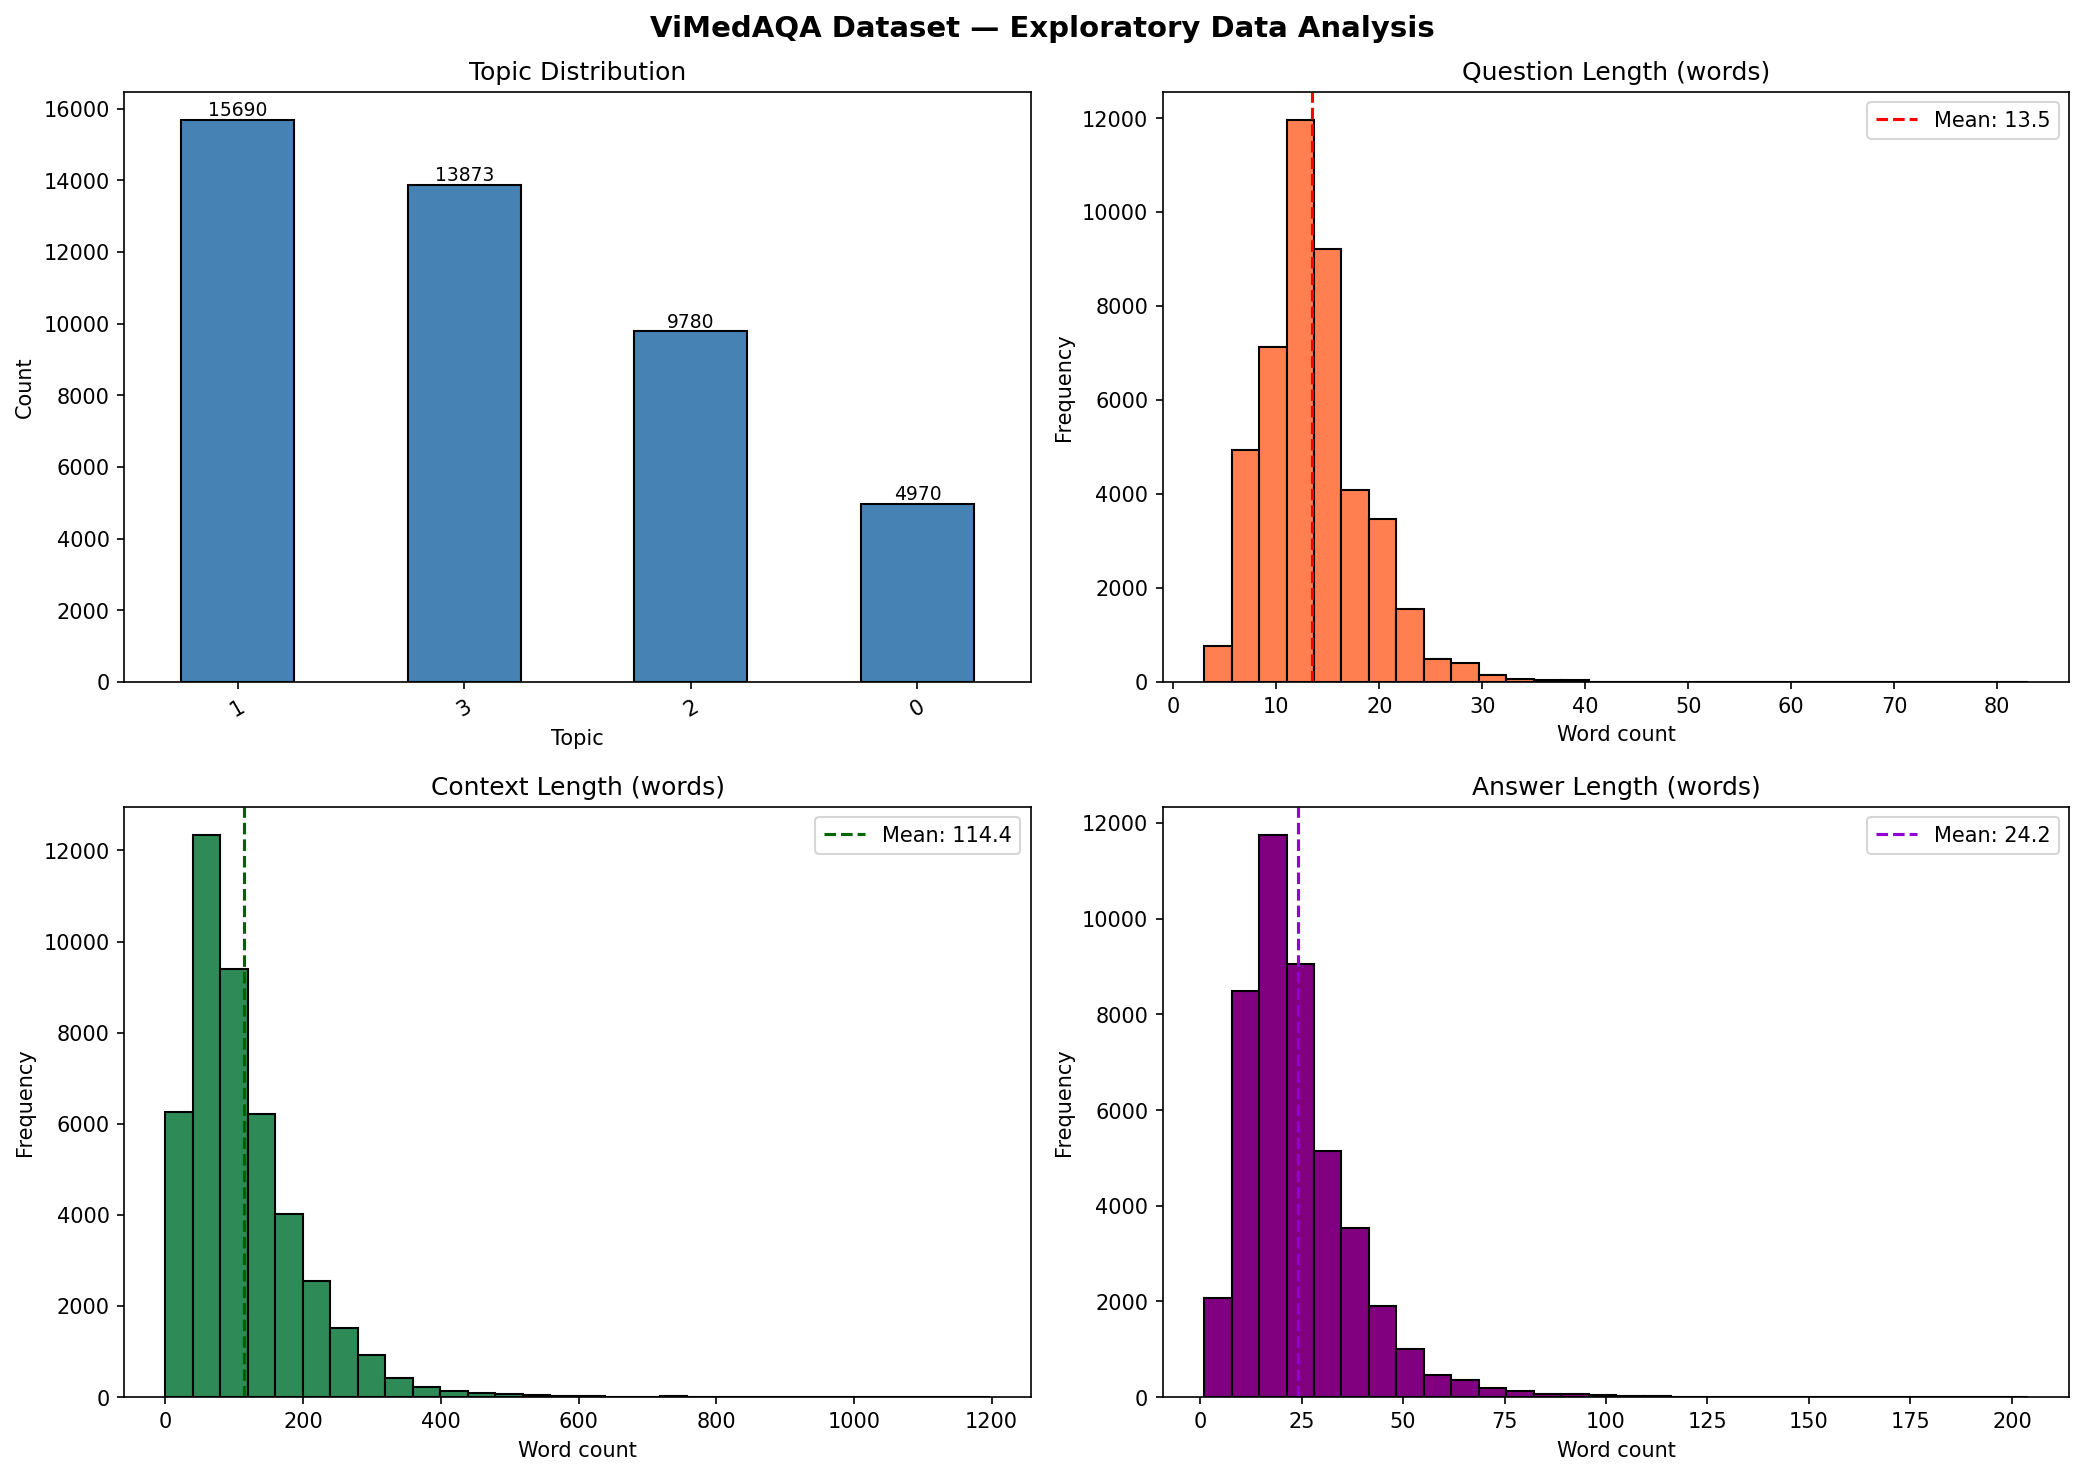
\includegraphics[width=0.85\textwidth]{figures/length_distributions.png}
    \caption{Phân phối độ dài câu hỏi, ngữ cảnh và câu trả lời trong bộ dữ liệu ViMedAQA}
    \label{fig:length_dist}
\end{figure}

Từ biểu đồ Hình~\ref{fig:length_dist}, có thể quan sát thấy phân phối độ dài câu hỏi tập trung rất ngắn (đa số dưới 50 từ), phù hợp với hành vi đặt câu hỏi tự nhiên của người bệnh. Câu trả lời cũng được tối ưu hóa độ dài trong khoảng từ 20 đến 100 từ nhằm đảm bảo tính súc tích, tránh lan man. Ngược lại, ngữ cảnh y học có phân phối trải rộng hơn và có đuôi dài (long-tail) lên đến hơn 500 từ. Phân phối này đòi hỏi các mô hình sinh chuỗi phải có khả năng biểu diễn ngữ cảnh dài hiệu quả mà không bị suy giảm khả năng tập trung (attention distraction).

\section{Chia tập dữ liệu phân tầng (Stratified Split)}
Để đảm bảo quá trình huấn luyện và đánh giá không bị sai lệch do mất cân bằng phân phối giữa các tập dữ liệu con, chúng tôi áp dụng kỹ thuật chia dữ liệu phân tầng (\textbf{Stratified Split}) dựa trên nhãn kết hợp giữa chủ đề y khoa (\texttt{topic}) và loại câu hỏi (\texttt{question\_type}) với giá trị seed cố định là \texttt{42}. Quy trình này giúp giữ nguyên tỷ lệ phân phối của từng lớp chủ đề trong cả ba tập huấn luyện, kiểm định và kiểm thử, ngăn ngừa hiện tượng dịch chuyển phân phối (distribution shift) vốn là tác nhân chính gây suy giảm độ ổn định của mô hình khi triển khai thực tế. Quy trình dọn dẹp dữ liệu cũng đã loại bỏ hoàn toàn các mẫu trùng lặp và rò rỉ dữ liệu (data leakage) giữa tập huấn luyện và tập kiểm thử, đảm bảo kết quả thực nghiệm hoàn toàn khách quan.
\chapter{Phương pháp nghiên cứu}
\section{Tổng quan quy trình nghiên cứu}
Đề tài được xây dựng trên một quy trình nghiên cứu gồm tám phase được thiết kế chặt chẽ và nhất quán theo đúng tài liệu thiết kế \texttt{PIPELINE\_ViMedAQA.md}:
\begin{enumerate}
    \item \textbf{Project Setup \& Exploratory Data Analysis (EDA):} Thiết lập môi trường huấn luyện, dọn dẹp dữ liệu trùng lặp và tiến hành khảo sát thống kê mô tả.
    \item \textbf{Baseline Zero-shot (Gemini):} Thiết lập hiệu năng tham chiếu trên mô hình ngôn ngữ lớn thương mại thông qua Groq API \texttt{Llama-3.3-70B-versatile}.
    \item \textbf{Fine-tuning ViT5:} Tinh chỉnh mô hình sinh chuỗi chuyên biệt tiếng Việt ViT5-base.
    \item \textbf{Fine-tuning BARTpho:} Tinh chỉnh mô hình Sequence-to-Sequence BARTpho-word phục vụ đối sánh chéo.
    \item \textbf{Unified Evaluation:} Đánh giá đồng bộ hiệu năng của tất cả các mô hình trên cùng tập test và cùng bộ độ đo chuẩn hóa.
    \item \textbf{Error Analysis \& Ablation Study:} Phân tích định tính các lỗi tiêu biểu của mô hình và thực hiện nghiên cứu ablation study trên các chiến lược giải mã.
    \item \textbf{Model Publishing:} Đóng gói và đẩy trọng số mô hình lên HuggingFace Hub.
    \item \textbf{Gradio Web RAG Interface:} Xây dựng ứng dụng hỏi đáp kết hợp tìm kiếm ngữ cảnh y học và triển khai demo lên HuggingFace Spaces.
\end{enumerate}

\section{Kiến trúc sinh câu trả lời dựa trên Retrieval-Augmented Generation (RAG)}
Để giải quyết triệt để hai thách thức lớn nhất của các mô hình ngôn ngữ nhỏ (Small Language Models - SLMs) trong miền y khoa là giới hạn tri thức nền (parametric memory) và hiện tượng ảo giác thông tin (factual hallucination), đề tài nghiên cứu và triển khai hệ thống hỏi đáp theo kiến trúc tinh chỉnh \textbf{RAG (Retrieval-Augmented Generation)}. Kiến trúc đề xuất là một pipeline đa tầng, được kiểm duyệt thông qua 3 cấu phần chính:

\subsection{Cấu phần truy xuất song song (Hybrid Retrieval)}
Khi nhận được một câu hỏi y tế $q$ từ người dùng, hệ thống sẽ chuẩn hóa (chuyển chữ thường, xóa khoảng trắng thừa) và tiến hành tìm kiếm trên tập tri thức y học độc lập (\texttt{medical\_corpus.json}). Nhằm tận dụng tối đa thế mạnh của các phương pháp tìm kiếm, hệ thống kích hoạt đồng thời hai cơ chế truy xuất:
\begin{itemize}
    \item \textbf{Truy xuất thưa (Sparse Retrieval - BM25Okapi):} Câu hỏi được tách từ tiếng Việt qua thư viện \texttt{PyViTokenizer} và đưa vào thuật toán BM25Okapi để tính điểm tương quan dựa trên tần suất từ khóa. Phương pháp này xuất sắc trong việc bắt chính xác các từ khóa "cứng" như tên bệnh lý hoặc tên biệt dược. Kết quả trả về top $50$ tài liệu tốt nhất.
    \item \textbf{Truy xuất dày đặc (Dense Retrieval - Bi-Encoder + FAISS):} Hệ thống sử dụng mô hình biểu diễn ngữ nghĩa \texttt{bkai-foundation-models/vietnamese-bi-encoder} để ánh xạ câu hỏi vào không gian vector $384$ chiều. Vector này được chuẩn hóa $L_2$ và tìm kiếm độ tương đồng trong không gian \textbf{FAISS IndexFlatIP} (sử dụng Inner Product). Phương pháp này giúp nắm bắt ý nghĩa khái niệm sâu sắc ngay cả khi từ ngữ bề mặt không trùng khớp. Kết quả cũng trả về top $50$ tài liệu có khoảng cách gần nhất.
\end{itemize}

\subsection{Cấu phần lai ghép và tái xếp hạng (Fusion \& Re-ranking)}
Để tổng hợp và đánh giá lại kết quả từ hai bộ tìm kiếm độc lập, hệ thống áp dụng luồng xử lý hai bước nhằm chắt lọc ra các ngữ cảnh chính xác nhất:
\begin{enumerate}
    \item \textbf{Lai ghép thứ hạng (Reciprocal Rank Fusion - RRF):} Các tài liệu ứng viên từ BM25 và FAISS được gộp lại và tính điểm trọng số chéo. Hệ thống thiết lập trọng số ưu tiên ngữ nghĩa cao hơn ($w_{faiss} = 0.65$, $w_{bm25} = 0.35$) với hằng số làm mượt $K = 50$. Điểm RRF của mỗi tài liệu $d$ được tính theo công thức:
    $$RRF\_Score(d) = \frac{0.35}{50 + rank_{bm25}(d)} + \frac{0.65}{50 + rank_{faiss}(d)}$$
    Thuật toán tiến hành sắp xếp và chọn ra top $50$ tài liệu tiềm năng nhất từ danh sách lai ghép.
    
    \item \textbf{Tái xếp hạng và lọc nhiễu (Cross-Encoder):} Top $50$ ứng viên tiếp tục được đưa qua mô hình \texttt{mmarco-mMiniLMv2-L12-H384-v1}. Khác với Bi-Encoder, Cross-Encoder tương tác chéo trực tiếp cặp (Câu hỏi, Ngữ cảnh) để sinh ra giá trị thô (logit). Giá trị này được biến đổi qua hàm kích hoạt Sigmoid ($\sigma$) để tính toán độ tin cậy thực tế:
    $$prob\_score = \sigma(logit) = \frac{1}{1 + e^{-logit}}$$
    Hệ thống thiết lập một chốt chặn an toàn với ngưỡng $\tau = 0.4$. Các ngữ cảnh có $prob\_score < \tau$ sẽ bị đánh dấu là dữ liệu nhiễu và lập tức bị loại bỏ. Hệ thống sẽ lấy top-$K$ (mặc định $K=3$) ngữ cảnh vượt qua kiểm duyệt để chuyển sang bộ sinh.
\end{enumerate}

\subsection{Cấu phần sinh câu trả lời (Generator)}
Nếu không có ngữ cảnh nào vượt qua màng lọc kiểm duyệt, hệ thống kích hoạt cơ chế Fallback, tự động từ chối trả lời để đảm bảo an toàn y khoa. Ngược lại, tập ngữ cảnh sạch thu được sẽ được ghép nối với câu hỏi ban đầu $q$ theo cấu trúc Prompt nghiêm ngặt:
$$X = \text{``question: } q \text{ context: } c_1 \ . \ c_2 \ . \ \dots \ c_K\text{''}$$

\noindent Chuỗi $X$ được SentencePiece Tokenizer phân tách và đưa vào mô hình Sequence-to-Sequence \texttt{ViT5-base} (\texttt{ntthanh0307/vit5-vimedaq-medical-qa}). Quá trình giải mã tự hồi quy sử dụng thuật toán Beam Search với cấu hình tối ưu hiệu năng (số chùm \texttt{num\_beams=2}, hệ số phạt lặp \texttt{repetition\_penalty=1.5}, hệ số phạt độ dài \texttt{length\_penalty=2.0}). Các tham số này ép mô hình phải bám sát ngữ liệu đầu vào để sinh ra câu trả lời y tế minh bạch, chính xác và giảm thiểu rủi ro sinh từ vựng ảo giác.

\subsection{Sơ đồ kiến trúc tổng thể}
Dưới đây là sơ đồ kiến trúc tổng thể của dự án:

\begin{figure}[H]
    \centering
    \resizebox{\textwidth}{!}{% Đảm bảo co giãn đồng bộ toàn bộ sơ đồ vừa khít trang A4
\begin{tikzpicture}[
    font=\sffamily\small,
    >=Stealth,
    node distance=0.8cm and 0.8cm,
    % --- Styles cho các node con ---
    box/.style={rectangle, draw=black!60, thick, rounded corners, align=center, minimum width=3.8cm, minimum height=0.9cm, fill=white},
    db/.style={cylinder, draw=gray!80, thick, aspect=0.25, shape border rotate=90, align=center, fill=gray!10, minimum width=3.2cm, minimum height=1.2cm},
    diamondbox/.style={diamond, draw=red!60, thick, fill=white, aspect=2, inner sep=2pt, align=center},
    % --- Styles màu cho từng Khối ---
    col1/.style={box, draw=blue!60, fill=blue!5},
    col2/.style={box, draw=orange!60, fill=orange!5},
    col3/.style={box, draw=green!60!black, fill=green!5},
    col4/.style={box, draw=purple!60, fill=purple!5},
    title/.style={font=\bfseries, align=center}
]

% ==========================================
% KHỐI 1: PIPELINE XỬ LÝ DỮ LIỆU (ETL)
% ==========================================
\node[db] (c1_raw) {Dữ liệu y tế thô\\(VimedQA Raw)};
\node[col1, below=of c1_raw] (c1_clean) {Lọc trùng \&\\Làm sạch văn bản};
\node[col1, below=of c1_clean] (c1_chunk) {Chunking theo câu\\(Sentence-aware)};
\node[col1, below=of c1_chunk] (c1_meta) {Làm giàu Metadata\\([Keyword] Title)};
\node[col1, below=of c1_meta] (c1_json) {Tệp Corpus JSON\\(Sẵn sàng Index)};

\draw[->, thick] (c1_raw) -- (c1_clean);
\draw[->, thick] (c1_clean) -- (c1_chunk);
\draw[->, thick] (c1_chunk) -- (c1_meta);
\draw[->, thick] (c1_meta) -- (c1_json);

% ==========================================
% KHỐI 2: ĐÁNH CHỈ MỤC ĐA NHÁNH
% ==========================================
\node[col2, right=2.5cm of c1_clean] (c2_dense_model) {Bi-Encoder Model\\(vietnamese-sbert)};
\node[col2, below=of c2_dense_model] (c2_faiss) {FAISS Vector DB\\(Nhánh Dense)};

\node[col2, below=1.5cm of c2_faiss] (c2_sparse_model) {PyVi Tokenizer\\(Tách từ TV)};
\node[col2, below=of c2_sparse_model] (c2_bm25) {BM25 Index\\(Nhánh Sparse)};

\draw[->, thick] (c1_json.east) -- ++(1cm,0) |- (c2_dense_model.west);
\draw[->, thick] (c1_json.east) -- ++(1cm,0) |- (c2_sparse_model.west);

\draw[->, thick] (c2_dense_model) -- (c2_faiss);
\draw[->, thick] (c2_sparse_model) -- (c2_bm25);

% ==========================================
% KHO LƯU TRỮ CỤC BỘ (HUGGING FACE)
% ==========================================
\node[db, right=1.8cm of c2_faiss, yshift=-2cm, fill=teal!10, draw=teal!80] (hf_storage) {Tệp tin cục bộ\\(Hugging Face Space)};

% Biểu diễn thao tác Upload file thủ công/Git LFS
\draw[->, thick, dashed] (c2_faiss.east) -| node[midway,above,xshift=-1.5cm,font=\scriptsize\ttfamily] {faiss\_index.bin} (hf_storage.north);
\draw[->, thick, dashed] (c2_bm25.east) -| node[below, xshift=-1.5cm,font=\scriptsize\ttfamily] {bm25\_index.pkl} (hf_storage.south);

% ==========================================
% KHỐI 3: LUỒNG RAG CỐT LÕI (RUN-TIME)
% ==========================================
\node[col3, right=6.5cm of c2_dense_model, yshift=1.5cm] (c3_user) {Người dùng\\(Gửi câu hỏi)};
\node[col3, below=of c3_user] (c3_prep) {Chuẩn hóa \&\\Từ đồng nghĩa};
\node[col3, below=of c3_prep] (c3_hybrid) {Truy xuất song song\\(Hybrid Search)};
\node[col3, below=of c3_hybrid] (c3_rrf) {Hợp nhất \&\\Nội suy điểm (RRF)};
\node[col3, below=of c3_rrf] (c3_cross) {Cross-Encoder\\(Chấm điểm \& Rerank)};
\node[diamondbox, below=0.5cm of c3_cross] (c3_thresh) {Score > 0.4?};

\draw[->, thick] (c3_user) -- (c3_prep);
\draw[->, thick] (c3_prep) -- (c3_hybrid);

% Ứng dụng đọc file tĩnh trực tiếp từ ổ cứng của Hugging Face
\draw[->,thick] (hf_storage.east)--(c3_hybrid.west);

\draw[->, thick] (c3_hybrid) -- (c3_rrf);
\draw[->, thick] (c3_rrf) -- (c3_cross);
\draw[->, thick] (c3_cross) -- (c3_thresh);

% ==========================================
% KHỐI 4: TỔNG HỢP & HIỂN THỊ UI
% ==========================================
% �� Đà LOẠI BỎ PROMPT ENGINEERING, NỐI ĐẠT TRỰC TIẾP VÀO ViT5
\node[col4, right=2cm of c3_hybrid] (c4_vit5) {ViT5 Seq2Seq\\(Tổng hợp câu trả lời)};
\node[col4, below=1cm of c4_vit5] (c4_out) {Giao diện Gradio\\(Hiển thị kết quả)};
\node[col4, below=1cm of c4_out] (c4_fallback) {Fallback\\(Cảnh báo từ chối)};

% Điều hướng từ Diamond (Pass đi vào LLM, Fall đi vào Fallback)
\draw[->, thick] (c3_thresh.east) -- ++(1,0) |- node[above, xshift=0.5cm, font=\bfseries] {Đạt} (c4_vit5.west);
\draw[->, thick] (c3_thresh.south)--++(0,-0.45cm)--++(5.9cm,0)node[midway,above, font=\bfseries, xshift=-0.2cm] {Thấp} --++(0,2cm)--(c4_fallback.south);

\draw[->, thick] (c4_vit5) -- (c4_out);
\draw[->, thick, dashed] (c4_fallback) |- (c4_out.south);


%\draw[->, thick, dashed, draw=blue!50] (c4_out.east) -- ++(-1.5cm,0) |- (c3_user.west);
% Thêm nhãn cho đường phản hồi nếu cần: node[near start,above,rotate=90] {Gửi câu hỏi tiếp}

% ==========================================
% VẼ KHUNG BACKGROUND CHO CÁC KHỐI
% ==========================================
\begin{scope}[on background layer]
    % Background Khối 1
    \node[rectangle, draw=blue!80, fill=blue!5, thick, rounded corners, inner sep=15pt, fit=(c1_raw) (c1_json)] (bg1) {};
    \node[title, text=blue!80!black, anchor=south] at (bg1.north) {KHỐI 1: PIPELINE XỬ LÝ\\DỮ LIỆU (ETL)};
    
    % Background Khối 2
    \node[rectangle, draw=orange!80, fill=orange!5, thick, rounded corners, inner sep=15pt, fit=(c2_dense_model) (c2_bm25)] (bg2) {};
    \node[title, text=orange!80!black, anchor=south] at (bg2.north) {KHỐI 2: ĐÁNH CHỈ MỤC\\ĐA NHÁNH (INDEXING)};
    
    % Background Khối 3
    \node[rectangle, draw=green!80!black, fill=green!5, thick, rounded corners, inner sep=15pt, fit=(c3_user) (c3_thresh)] (bg3) {};
    \node[title, text=green!60!black, anchor=south] at (bg3.north) {KHỐI 3: LUỒNG RAG\\CỐT LÕI (RUN-TIME)};
    

    \node[rectangle, draw=purple!80, fill=purple!5, thick, rounded corners, inner sep=15pt, fit=(c4_vit5) (c4_fallback) (c4_out)] (bg4) {};
    \node[title, text=purple!80!black, anchor=south] at (bg4.north) {KHỐI 4: TỔNG HỢP\\\& HIỂN THỊ UI};
\end{scope}

\end{tikzpicture}
    }
    \caption{Sơ đồ kiến trúc tổng thể của hệ thống ViMedAQA}
    \label{fig:architecture_diagram}
\end{figure}

\section{Quy trình huấn luyện và tối ưu hóa Seq2Seq}
Quá trình tinh chỉnh (fine-tuning) hai mô hình chính ViT5-base \cite{phan2022vit5} và BARTpho-word \cite{tran2021bartpho} sử dụng hàm mất mát âm log-likelihood (Negative Log-Likelihood - NLL) trên từng token của chuỗi đáp án mục tiêu:
\begin{equation}
  \mathcal{L}(\theta) = -\sum_{t=1}^{T}\log p_\theta(a_t \mid a_{<t}, X)
\end{equation}
Trong đó $\theta$ đại diện cho các trọng số mạng nơ-ron được tối ưu hóa.

Để đảm bảo quá trình đối sánh chéo diễn ra công bằng, chúng tôi thiết kế quy trình huấn luyện đồng bộ về mặt kích thước batch hiệu dụng (Effective Batch Size), thuật toán tối ưu hóa và số lượng epoch huấn luyện. Tuy nhiên, do kiến trúc tokenizer và dung lượng bộ nhớ của hai mô hình có sự khác biệt lớn, các siêu tham số kỹ thuật được tinh chỉnh linh hoạt nhằm tránh lỗi tràn bộ nhớ (Out of Memory - OOM) trên GPU Nvidia T4 ($16$GB VRAM) của Google Colab. Bảng~\ref{tab:training_configs} tổng hợp chi tiết cấu hình huấn luyện thực tế của các mô hình.

\begin{table}[H]
\centering
\caption{Cấu hình siêu tham số huấn luyện thực tế trong đề tài}
\label{tab:training_configs}
\resizebox{\textwidth}{!}{%
\begin{tabular}{lcc}
\toprule
\textbf{Siêu tham số} & \textbf{Mô hình chính (ViT5-base)} & \textbf{Mô hình đối sánh (BARTpho-word)} \\
\midrule
Kiến trúc cơ sở & T5 (Text-to-Text) \cite{raffel2020t5} & BART (Seq2Seq Autoencoder) \cite{lewis2020bart} \\
Dung lượng mô hình & 220M parameters & 228M parameters \\
Kích thước Batch huấn luyện & per-device batch size = 4 & per-device batch size = 2 \\
Gradient Accumulation Steps & 4 steps & 8 steps \\
\textbf{Batch size hiệu dụng} & \textbf{16} & \textbf{16} \\
Tối ưu hóa (Optimizer) & AdamW ($\beta_1=0.9, \beta_2=0.999$) & AdamW ($\beta_1=0.9, \beta_2=0.999$) \\
Tốc độ học (Learning Rate) & $3 \times 10^{-4}$ & $3 \times 10^{-4}$ \\
Lịch trình giảm tốc độ học & Linear Warmup ($10\%$ steps) & Linear Warmup ($10\%$ steps) \\
Số Epoch huấn luyện & 5 epochs & 5 epochs \\
Độ dài đầu vào cực đại & 512 tokens & 1024 tokens \\
Độ dài đầu ra cực đại & 128 tokens & 256 tokens \\
Kiểu dữ liệu số thực & mixed precision (\texttt{fp16}) & mixed precision (\texttt{fp16}) \\
Gradient Checkpointing & Tắt & \textbf{Bật (Bắt buộc để tránh OOM)} \\
\bottomrule
\end{tabular}%
}
\end{table}

Việc duy trì kích thước batch hiệu dụng bằng $16$ giúp hướng gradient di chuyển ổn định trong không gian tham số, hỗ trợ cả hai mô hình hội tụ tốt. Cơ chế \textbf{Gradient Checkpointing} được kích hoạt bắt buộc cho BARTpho-word để đánh đổi tài nguyên tính toán lấy dung lượng bộ nhớ, cho phép mô hình xử lý chuỗi đầu vào dài lên tới $1024$ tokens mà không gặp sự cố phần cứng. Quá trình huấn luyện cũng tích hợp cơ chế lưu checkpoint tự động và lưu nhật ký huấn luyện định kỳ lên Google Drive để phòng ngừa rủi ro mất kết nối đột ngột trong môi trường Colab. Checkpoint cuối cùng được lựa chọn dựa trên chỉ số tổn thất kiểm định (\texttt{eval\_loss}) thấp nhất trên tập validation.
\chapter{Thực nghiệm và đánh giá}
\section{Thiết lập thực nghiệm}
Tất cả các thực nghiệm đánh giá hiệu năng đều được thực hiện nhất quán trên cùng tập kiểm thử độc lập (\texttt{test.json}) gồm $2.356$ mẫu dữ liệu. Đối với các mô hình fine-tuned (ViT5-base và BARTpho-word), quá trình suy luận (inference) được thực hiện với chiến lược giải mã mặc định là Beam Search với kích thước chùm $B=4$ để đảm bảo chất lượng sinh tối ưu. Đối với baseline zero-shot (Llama-3.3-70B-versatile), chúng tôi gọi API Groq với cấu hình nhiệt độ (temperature) bằng $0.0$ nhằm loại bỏ tính ngẫu nhiên, tập trung hoàn toàn vào khả năng suy luận logic y khoa. Toàn bộ các kết quả dự đoán (prediction) được xuất ra tệp định dạng JSON đồng bộ để tính toán các độ đo định lượng mà không bị sai lệch về mặt kỹ thuật.

\section{Các độ đo đánh giá định lượng}
Để đánh giá toàn diện năng lực của các mô hình từ mức độ trùng khớp từ ngữ bề mặt đến độ tương đồng ngữ nghĩa sâu sắc, đề tài sử dụng ba nhóm độ đo tiêu chuẩn trong xử lý ngôn ngữ tự nhiên:

\subsection{ROUGE (Recall-Oriented Understudy for Gisting Evaluation)}
\cite{lin2004rouge}
ROUGE đánh giá mức độ trùng khớp của chuỗi văn bản thông qua ba chỉ số chính:
\begin{itemize}
    \item \textbf{ROUGE-1:} Tính toán tỉ lệ trùng khớp unigram (từ đơn), đo lường mức độ bảo toàn các thực thể y học đơn lẻ.
    \item \textbf{ROUGE-2:} Tính toán tỉ lệ trùng khớp bigram (cặp từ liền kề), phản ánh khả năng duy trì các thuật ngữ ghép y khoa chính xác.
    \item \textbf{ROUGE-L:} Dựa trên chuỗi con chung dài nhất (Longest Common Subsequence - LCS), phản ánh khả năng bảo toàn cấu trúc cú pháp tự nhiên của câu trả lời.
\end{itemize}

\subsection{BLEU (Bilingual Evaluation Understudy)}
\cite{papineni2002bleu}
BLEU-4 đo lường độ chính xác n-gram (với $n$ từ $1$ đến $4$) có phạt độ dài (brevity penalty). Chỉ số này phản ánh độ chính xác của các phân đoạn văn bản được sinh ra so với câu tham chiếu mục tiêu.

\subsection{BERTScore}
\cite{zhang2020bertscore}
BERTScore tận dụng biểu diễn ngữ nghĩa dày đặc của mô hình ngôn ngữ lớn tiền huấn luyện (\texttt{multilingual-BERT}) để tính toán độ tương đồng cosine giữa các token biểu diễn. BERTScore có ưu thế tuyệt đối trong bài toán sinh văn bản trừu tượng vì nó ghi nhận chính xác các câu trả lời đồng nghĩa mặc dù sử dụng từ ngữ bề mặt khác biệt hoàn toàn với câu tham chiếu.

\section{Bảng so sánh kết quả thực nghiệm tổng thể}
Kết quả thực nghiệm định lượng chi tiết của các mô hình trên tập kiểm thử được tổng hợp và đối sánh tại Bảng~\ref{tab:comparison}.

\begin{table}[H]
\centering
\caption{Bảng đối sánh hiệu năng định lượng giữa các mô hình trên tập kiểm thử ViMedAQA}
\label{tab:comparison}
\resizebox{\textwidth}{!}{%
\begin{tabular}{lccccc}
\toprule
\textbf{Mô hình} & \textbf{ROUGE-1} & \textbf{ROUGE-2} & \textbf{ROUGE-L} & \textbf{BLEU-4} & \textbf{BERTScore F1} \\
\midrule
Llama-3.3-70B-versatile (zero-shot) & 0,7285 & \textbf{0,6257} & 0,6664 & 0,4684 & \textbf{0,8757} \\
ViT5-base (fine-tuned) & 0,7318 & 0,6153 & 0,6680 & \textbf{0,5005} & 0,8752 \\
BARTpho-word (fine-tuned) & \textbf{0,7327} & 0,6185 & \textbf{0,6681} & 0,2794 & 0,8230 \\
\bottomrule
\end{tabular}%
}
\end{table}

\section{Biện luận khoa học sâu sắc về kết quả thực nghiệm}
Từ kết quả tại Bảng~\ref{tab:comparison}, chúng tôi rút ra ba luận điểm phân tích học thuật quan trọng:

\subsection{Đặc tính phân tách từ của Tokenizer tác động lên độ đo BLEU-4}
Một quan sát cực kỳ nổi bật là mặc dù mô hình \textbf{BARTpho-word} đạt điểm số ROUGE-1 (\textbf{0,7327}) và ROUGE-L (\textbf{0,6681}) cao nhất trong tất cả các mô hình, chỉ số BLEU-4 của nó lại sụt giảm nghiêm trọng xuống mức cực thấp (\textbf{0,2794}), so với mức \textbf{0,5005} của ViT5-base. Đây là một hiện tượng kỹ thuật đặc thù cần được giải thích rõ ràng. 

BARTpho-word được tiền huấn luyện trên dữ liệu tiếng Việt đã được phân tách từ bằng công cụ tokenizer mức từ (word-level). Do đó, câu trả lời sinh ra bởi BARTpho chứa các dấu gạch dưới (\texttt{\_}) để liên kết các âm tiết trong một từ ghép (ví dụ: \texttt{chấn\_thương\_sọ\_não}, \texttt{tuyến\_yên}). Tuy nhiên, bộ tính toán độ đo BLEU-4 chuẩn hóa lại thực hiện tách từ dựa trên khoảng trắng mặc định mà không có cơ chế xử lý dấu gạch dưới y khoa. Sự lệch pha này làm mất đi khả năng trùng khớp n-gram cao (từ 3-gram đến 4-gram), dẫn đến điểm BLEU-4 bị phạt nặng nề mặc dù về mặt ngữ nghĩa và cấu trúc câu (phản ánh qua ROUGE-L), BARTpho-word hoàn toàn tương đương, thậm chí nhỉnh hơn ViT5-base. Phát hiện này nhấn mạnh rằng không nên áp dụng BLEU-4 một cách rập khuôn để đánh giá các mô hình tiếng Việt sử dụng tokenizer cấp từ nếu không có bước tiền xử lý chuẩn hóa khoảng trắng ngược lại.

\subsection{Ưu thế ngữ nghĩa của mô hình ngôn ngữ lớn (LLM)}
Mặc dù là mô hình zero-shot hoàn toàn không được huấn luyện trên dữ liệu ViMedAQA, \textbf{Llama-3.3-70B-versatile} đạt điểm số BERTScore F1 cao nhất (\textbf{0,8757}) và ROUGE-2 vượt trội (\textbf{0,6257}). Điều này chứng minh sức mạnh của tri thức nền tảng y học khổng lồ (parametric knowledge) bên trong mô hình $70$ tỷ tham số. Llama-3.3 có khả năng diễn đạt các khái niệm y học cực kỳ chính xác và linh hoạt. Tuy nhiên, do tính chất zero-shot, phong cách hành văn của nó không bám sát hoàn hảo cấu trúc câu tham chiếu của ViMedAQA, dẫn đến điểm ROUGE-1 và ROUGE-L thấp hơn một chút so với hai mô hình sinh chuỗi được fine-tune trực tiếp.

\subsection{Năng lực vượt trội của ViT5-base trong bài toán sinh câu trả lời tiếng Việt}
Mô hình \textbf{ViT5-base} thể hiện sự cân bằng hoàn hảo trên tất cả các độ đo. Nó đạt điểm BLEU-4 cao nhất (\textbf{0,5005}) và chỉ số BERTScore F1 (\textbf{0,8752}) tương đương với siêu mô hình Llama-3.3-70B. Điều này chứng minh rằng việc tinh chỉnh một mô hình nhỏ chuyên biệt tiếng Việt ($220$M tham số) trên tập dữ liệu nội miền chất lượng cao hoàn toàn có khả năng tiệm cận hoặc vượt qua các mô hình ngôn ngữ khổng lồ thương mại trong một tác vụ chuyên biệt, tạo tiền đề cho việc triển khai ứng dụng y khoa chi phí thấp và bảo mật dữ liệu cao.

\section{Phân tích hiệu năng chi tiết theo chủ đề y khoa}
Để xác định mức độ ổn định của mô hình chính ViT5-base trên các miền tri thức y khoa khác nhau, chúng tôi tiến hành phân tích hiệu năng chi tiết theo từng lớp chủ đề y học độc lập. Kết quả phân tích được thể hiện tại Bảng~\ref{tab:per_topic}.

\begin{table}[H]
\centering
\caption{Phân tích chi tiết chỉ số ROUGE-L của mô hình ViT5-base theo từng chủ đề y khoa}
\label{tab:per_topic}
\resizebox{\textwidth}{!}{%
\begin{tabular}{lcc}
\toprule
\textbf{Chủ đề y học (Topic ID)} & \textbf{Số lượng mẫu kiểm thử ($n$)} & \textbf{ROUGE-L đạt được} \\
\midrule
Chủ đề 0 - diseases & 229 & 0,6528 \\
Chủ đề 1 - medicine & 780 & 0,6274 \\
Chủ đề 2 - drug & 588 & \textbf{0,7007} \\
Chủ đề 3 - body-part & 751 & 0,6920 \\
\bottomrule
\end{tabular}%
}
\end{table}

Bảng~\ref{tab:per_topic} chỉ ra rằng hiệu năng có sự dao động nhẹ giữa các chủ đề. \textbf{Chủ đề 2} đạt kết quả cao nhất (\textbf{0,7007}), tiếp theo là \textbf{Chủ đề 3} (\textbf{0,6920}). Ngược lại, \textbf{Chủ đề 1} mặc dù có số lượng mẫu rất lớn ($780$ mẫu) nhưng chỉ đạt chỉ số ROUGE-L thấp nhất (\textbf{0,6274}). Điều này chứng minh rằng độ khó của các chủ đề y khoa không chỉ phụ thuộc vào số lượng dữ liệu huấn luyện, mà phụ thuộc nhiều vào mức độ phức tạp của các thuật ngữ chuyên ngành và tính chất trừu tượng của câu trả lời trong chuyên khoa đó (ví dụ: các câu hỏi chẩn đoán và điều trị lâm sàng phức tạp ở Chủ đề 1 luôn đòi hỏi sự lập luận phức tạp hơn so với việc mô tả công dụng dược phẩm hoặc vị học cổ truyền đơn giản ở Chủ đề 2). Việc nhận diện được các chuyên khoa yếu này giúp định hướng cho các nghiên cứu tiếp theo trong việc thu thập thêm dữ liệu chuyên sâu để bù đắp khoảng trống tri thức.
\chapter{Phân tích lỗi, ablation và triển khai}

\section{Đường cong học tập và sự hội tụ của mô hình}

Để đánh giá trực quan quá trình huấn luyện và theo dõi trạng thái của mô hình ViT5-base, sự biến thiên của hàm mất mát (\texttt{train\_loss}) và chỉ số ROUGE-L trên tập kiểm định (\texttt{eval\_rougeL}) được ghi nhận qua các bước cập nhật tham số. Biểu đồ đường cong học tập thực tế được minh họa tại Hình~\ref{fig:learning_curve}.



\begin{figure}[H]

    \centering

    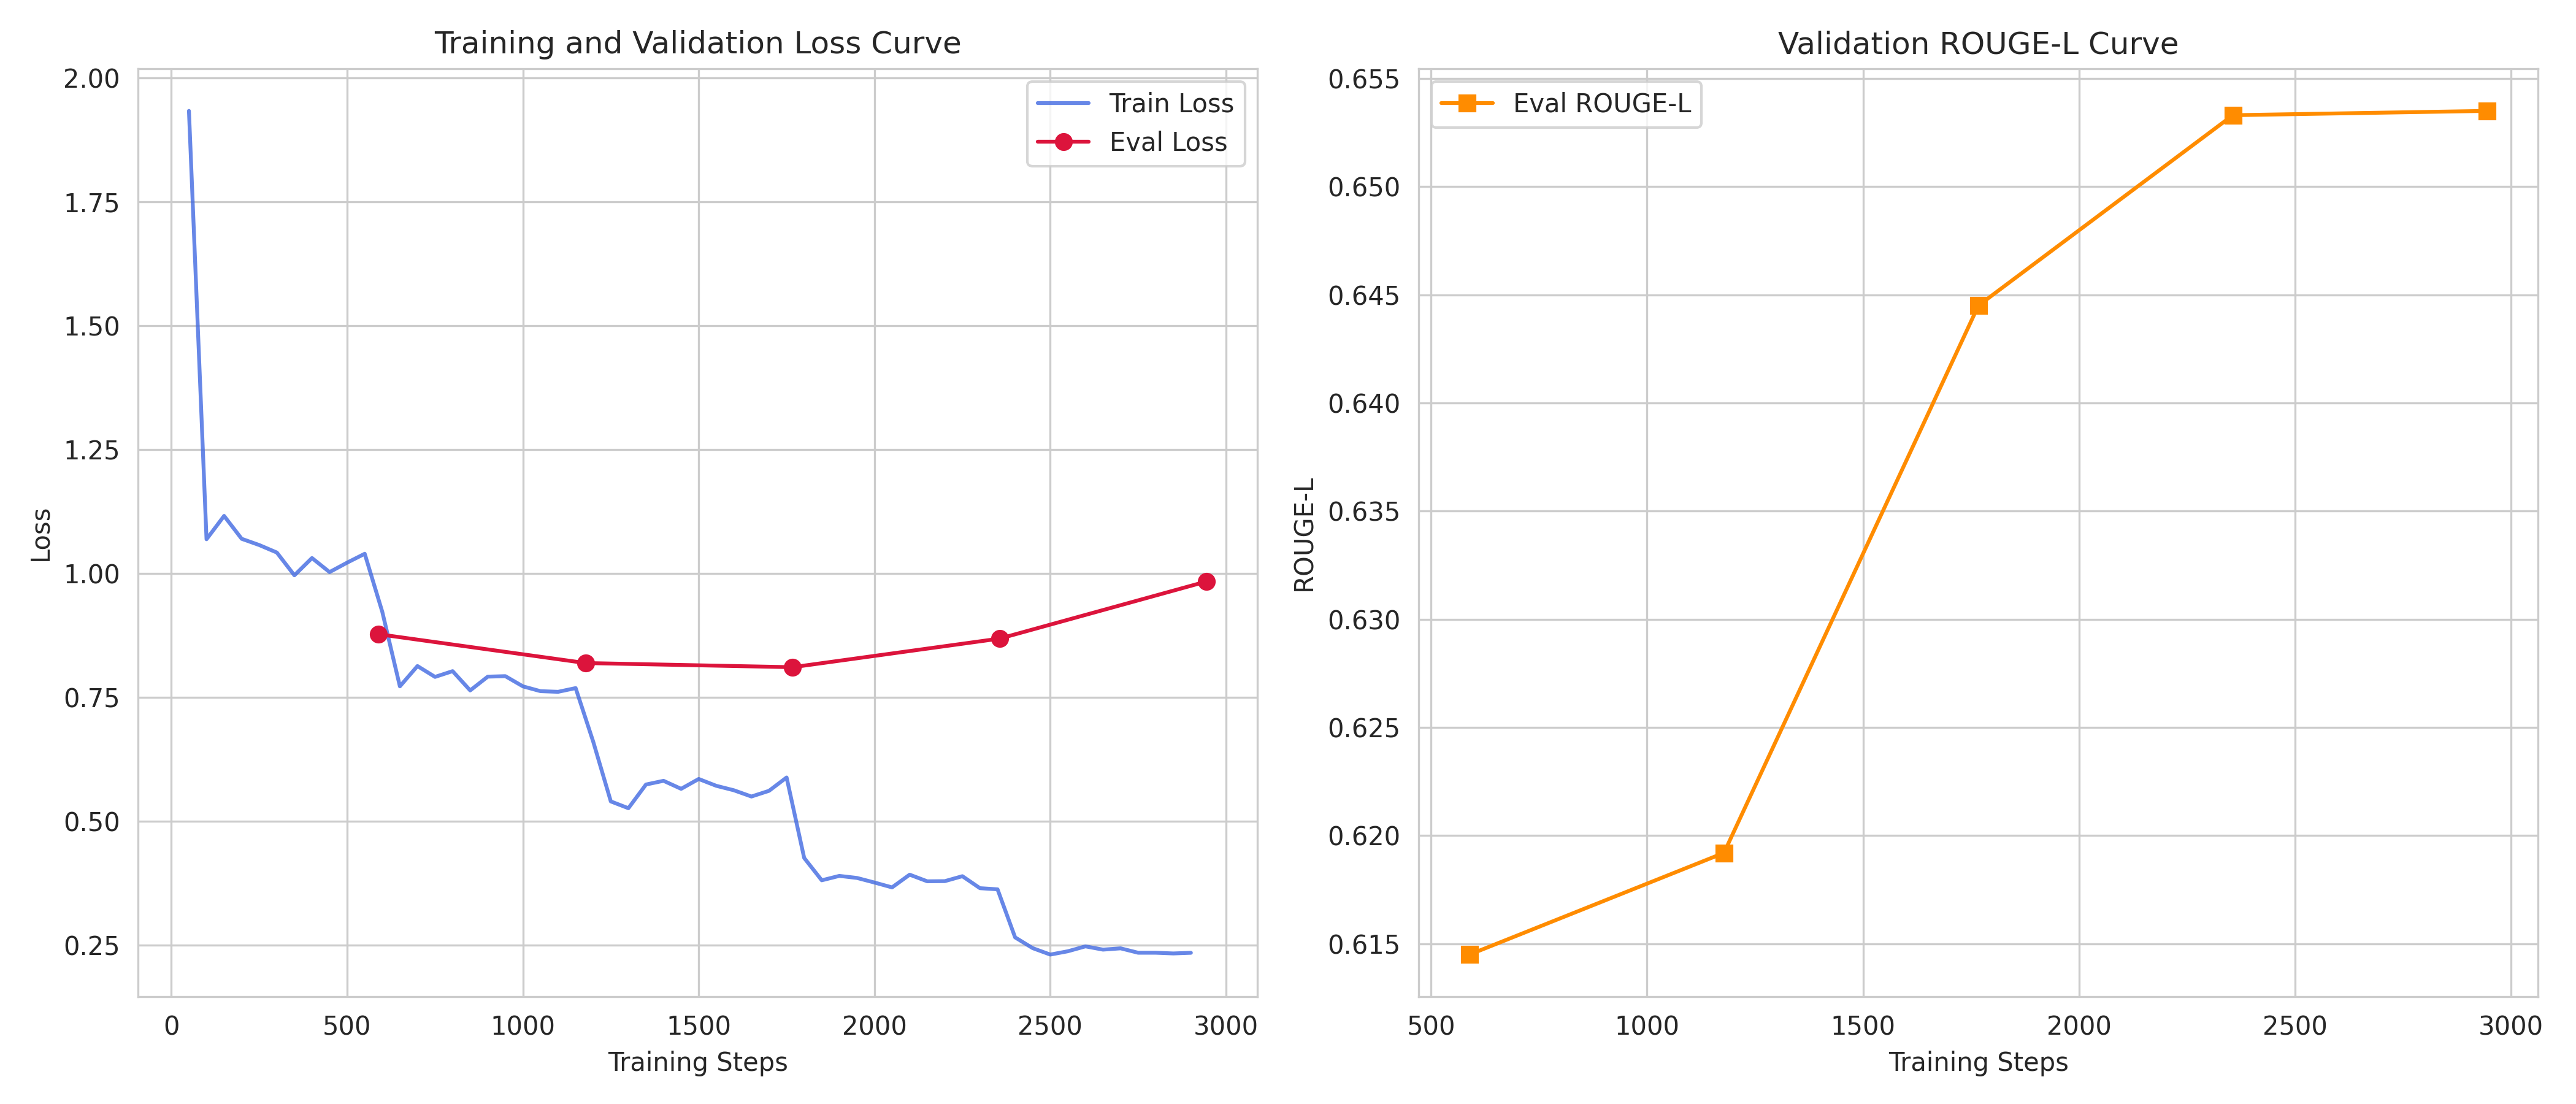
\includegraphics[width=0.85\textwidth]{figures/learning_curve_vit5.png}

    \caption{Đường cong học tập (Training/Validation Loss và Validation ROUGE-L) của mô hình ViT5-base}

    \label{fig:learning_curve}

\end{figure}



Từ Hình~\ref{fig:learning_curve}, hàm mất mát huấn luyện (Train Loss) có xu hướng giảm mạnh từ mức xấp xỉ $1,95$ và hội tụ về khoảng $0,25$ tại bước huấn luyện $3000$. Tuy nhiên, đối với tập kiểm định, hàm mất mát (Eval Loss) chỉ giảm đến giá trị cực tiểu khoảng $0,81$ tại bước $1800$ (tương đương epoch 3). Sau điểm này, Eval Loss bắt đầu tăng dần và chạm mức xấp xỉ $0,99$ ở bước $3000$, cho thấy mô hình đã bắt đầu xuất hiện hiện tượng quá khớp (overfitting) nhẹ. 
Song song đó, biểu đồ Validation ROUGE-L cho thấy hiệu suất chắp nối ngữ nghĩa bắt đầu từ $0,6145$, tăng trưởng mạnh mẽ và đạt trạng thái bão hòa (plateau) ở mức xấp xỉ $0,6536$ trong khoảng từ bước $2400$ đến bước $3000$. Sự bão hòa của chỉ số ROUGE-L kết hợp với đà tăng của Eval Loss ở giai đoạn cuối minh chứng rằng việc tiếp tục huấn luyện vượt quá bước $2400$ không mang lại giá trị gia tăng về chất lượng sinh văn bản, đồng thời việc hệ thống tự động thiết lập lưu \texttt{best\_model} dựa trên điểm ROUGE-L cao nhất thay vì Eval Loss thấp nhất là cần thiết để tối ưu hóa hiệu năng Abstractive QA.


\section{Nghiên cứu Ablation Study về chiến lược giải mã}
Chiến lược giải mã (decoding strategy) tại cấu phần generator có ảnh hưởng sống còn đến chất lượng văn bản y học sinh ra. Chúng tôi tiến hành nghiên cứu ablation study trên tập kiểm định (\texttt{val.json}) gồm $295$ mẫu để so sánh định lượng giữa hai phương pháp: giải mã tham lam (Greedy Decoding, $B=1$) và tìm kiếm chùm (Beam Search, $B=4$). Kết quả thực nghiệm được tổng hợp tại Bảng~\ref{tab:ablation_decoding}.

\begin{table}[H]
\centering
\caption{Kết quả Ablation Study về chiến lược giải mã trên tập kiểm định}
\label{tab:ablation_decoding}
\begin{tabular}{lccc}
\toprule
\textbf{Chiến lược giải mã} & \textbf{ROUGE-1} & \textbf{ROUGE-2} & \textbf{ROUGE-L} \\
\midrule
Greedy Decoding (beams=1) & 0,7188 & 0,5998 & 0,6527 \\
Beam Search (beams=4) & \textbf{0,7242} & \textbf{0,6069} & \textbf{0,6587} \\
\bottomrule
\end{tabular}
\end{table}

Kết quả tại Bảng~\ref{tab:ablation_decoding} chỉ ra rằng \textbf{Beam Search ($B=4$)} mang lại sự cải thiện đồng bộ trên tất cả các độ đo, cụ thể tăng khoảng \textbf{0,6\%} điểm ROUGE-L so với Greedy Decoding. Sự cải thiện này đạt được nhờ khả năng lưu giữ và đánh giá đồng thời nhiều giả thuyết dịch chuỗi tối ưu trên diện rộng, giúp mô hình tránh rơi vào các từ tối ưu cục bộ vốn dễ làm câu sinh ra bị cụt hoặc lặp từ. Tuy nhiên, Beam Search đòi hỏi chi phí tính toán và bộ nhớ lớn hơn. Trong các ứng dụng thực tế yêu cầu phản hồi tức thời với tài nguyên hạn chế, Greedy Decoding vẫn là một giải pháp thay thế rất khả thi nhờ tốc độ vượt trội mà không bị sụt giảm quá sâu về chất lượng.

\section{Phân tích định tính các trường hợp lỗi tiêu biểu (Failure Modes)}
Để hiểu rõ giới hạn nội tại và các điểm yếu y học của mô hình sinh, chúng tôi tiến hành phân tích định tính thủ công trên các mẫu dự đoán có điểm số thấp nhất từ tệp \texttt{worst\_10\_cases.csv}. Ba Failure Modes tiêu biểu đã được phát hiện và phân tích sâu sắc dưới góc độ y học lâm sàng:

\subsection{Lỗi lặp từ vô hạn (Repetitive Loop)}
\begin{tcolorbox}[colback=codebg, colframe=myblue, title={Ví dụ thực tế về lỗi lặp từ vô hạn do suy giảm tự hồi quy}]
\small\raggedright
\textbf{Câu hỏi:} Ngoài chấn thương đầu, còn có những nguyên nhân nào gây ra chóng mặt không?\par
\textbf{Tham chiếu:} Có rất nhiều nguyên nhân gây ra chóng mặt, như: rối loạn tiền đình, nhiễm trùng tai, tụt huyết áp, thiếu máu, sử dụng một số loại thuốc, v.v.\par
\textbf{Mô hình:} Có, chóng mặt có thể do chấn thương đầu, chấn thương đầu, chấn thương đầu, chấn thương đầu, chấn thương đầu, chấn thương đầu, chấn thương đầu, chấn thương đầu, chấn thương đầu, chấn thương đầu...
\end{tcolorbox}
\textbf{Biện luận y học và kỹ thuật:} Hiện tượng này xảy ra do sự suy giảm tự hồi quy (autoregressive degradation) của mô hình Seq2Seq khi sinh chuỗi dài. Khi phân phối xác suất của từ tiếp theo bị thống trị tuyệt đối bởi cụm từ vừa sinh ra trước đó (\textit{``chấn thương đầu''}), mô hình rơi vào trạng thái lặp vô hạn. Lỗi này cực kỳ nguy hiểm trong y tế vì nó triệt tiêu hoàn toàn thông tin hữu ích và gây trải nghiệm tồi tệ cho người dùng. Giải pháp khắc phục hiệu quả là thiết lập tham số hình phạt lặp từ khóa (\texttt{no\_repeat\_ngram\_size = 3}) hoặc áp dụng cơ chế giải mã đa dạng hóa (Contrastive Search) trong quá trình suy luận.

\subsection{Lỗi ảo tưởng thông tin lạc đề (Factual Hallucination \& Distraction)}
\begin{tcolorbox}[colback=codebg, colframe=myblue, title={Ví dụ thực tế về lỗi sinh thông tin ảo tưởng lạc đề}]
\small\raggedright
\textbf{Câu hỏi:} Nữ trinh tử và xấu hổ có đặc điểm gì giống nhau?\par
\textbf{Tham chiếu:} Cả hai đều thuộc họ Trinh nữ (Mimosaceae).\par
\textbf{Mô hình:} Cây xấu hổ có quả hình trứng hoặc hình bầu dục, có quả hơi cong, dài 7mm 10mm, đường kính khoảng 3mm, vỏ ngoài màu đen xám, có vằn nhăn, hai đầu tròn tày, một đầu có vết của cuống quả.
\end{tcolorbox}
\textbf{Biện luận y học và kỹ thuật:} Trong ví dụ này, mô hình đã tự sinh ra một mô tả cực kỳ chi tiết về quả của cây xấu hổ (được lưu giữ trong bộ nhớ tham số hoặc trích xuất từ phần ngữ cảnh dài liên quan đến cây xấu hổ). Tuy nhiên, mô hình hoàn toàn bỏ qua việc trả lời trọng tâm câu hỏi là chỉ ra \textit{điểm giống nhau} của hai loài thực vật y học (cùng thuộc họ Trinh nữ). Đây là lỗi mất tập trung ngữ cảnh (contextual distraction). Khi đối mặt với ngữ cảnh chứa quá nhiều chi tiết sinh học phức tạp, cơ chế Attention của mô hình bị quá tải và chọn lọc sai thông tin quan trọng. Điều này đòi hỏi retriever phải cắt gọt ngữ cảnh gọn gàng hơn trước khi đưa vào generator.

\subsection{Lỗi chi tiết quá mức gây sụt giảm độ đo (Overly Detailed Mismatch)}
\begin{tcolorbox}[colback=codebg, colframe=myblue, title={Ví dụ thực tế về câu trả lời y học chính xác bị chấm điểm thấp}]
\small\raggedright
\textbf{Câu hỏi:} Những bệnh lý nào tại tuyến yên có thể gây ra suy giảm tuyến thượng thận thứ phát?\par
\textbf{Tham chiếu:} U tuyến yên.\par
\textbf{Mô hình:} Những bệnh lý tại tuyến yên có thể gây ra suy giảm tuyến thượng thận thứ phát bao gồm: U tuyến yên hoặc vùng dưới đồi (một vùng ở não bộ), nhiễm trùng, ung thư, nhồi máu não, chấn thương sọ não, bất thường tuyến yên do đột biến gen.
\end{tcolorbox}
\textbf{Biện luận y học và kỹ thuật:} Đây là một trường hợp lỗi vô cùng đặc biệt. Về mặt y khoa học thuật, câu trả lời sinh ra bởi mô hình cực kỳ chính xác, đầy đủ và mang giá trị lâm sàng cao hơn rất nhiều so với câu trả lời tham chiếu quá ngắn gọn (\textit{``U tuyến yên''}). Tuy nhiên, do các độ đo ROUGE và BLEU chỉ tính toán dựa trên mức độ trùng khớp bề mặt n-gram của câu tham chiếu, mô hình bị chấm điểm ROUGE-L rất thấp (\textbf{0,1149}) và bị coi là lỗi \textit{Length Mismatch} (dài hơn $200\%$). Điều này vạch trần điểm hạn chế cốt lõi của các độ đo tự động truyền thống trong miền y tế - chúng thường phạt nặng những câu trả lời chi tiết và đầy đủ. Phát hiện này củng cố tầm quan trọng của việc sử dụng độ đo ngữ nghĩa BERTScore (đạt điểm rất cao trong trường hợp này) và kiểm chứng lâm sàng thủ công từ chuyên gia y tế.

\section{Công bố trọng số mô hình và mã nguồn mở}
Nhằm thúc đẩy khả năng tái lập nghiên cứu và đóng góp vào cộng đồng xử lý ngôn ngữ tự nhiên tiếng Việt, chúng tôi đã đóng gói toàn bộ trọng số mô hình tốt nhất (best checkpoint) của ViT5-base và đẩy lên hệ sinh thái HuggingFace Hub:
\begin{itemize}
    \item \textbf{Địa chỉ trọng số mô hình (HuggingFace Hub):} \href{https://huggingface.co/kimquoc/vit5-vimedaqa-medical-qa}{kimquoc/vit5-vimedaqa-medical-qa} hoặc \href{https://huggingface.co/ntthanh0307/vit5-vimedaq-medical-qa}{ntthanh0307/vit5-vimedaq-medical-qa}.
\end{itemize}
Trang model card đi kèm mô tả chi tiết thông số kiến trúc, bộ dữ liệu huấn luyện ViMedAQA, các chỉ số đánh giá thực nghiệm và đặc biệt là các điều khoản tuyên bố miễn trừ trách nhiệm pháp lý y khoa (medical disclaimer) bắt buộc khi ứng dụng mô hình vào thực tiễn.

\section{Triển khai ứng dụng Web Demo Gradio RAG}
Để trực quan hóa sức mạnh của mô hình trong thực tế, chúng tôi thiết kế và triển khai một ứng dụng web tương tác hoàn chỉnh dựa trên thư viện Gradio. Hệ thống được tích hợp kiến trúc Dense RAG tích hợp đầy đủ hai cấu phần Retriever (Bi-Encoder + FAISS) và Generator (ViT5-base) như đã mô tả ở Chương 3. Ảnh chụp màn hình giao diện thực tế của ứng dụng khi đang xử lý một truy vấn RAG y tế thành công được thể hiện tại Hình~\ref{fig:gradio_ui}.

\begin{figure}[H]
    \centering
    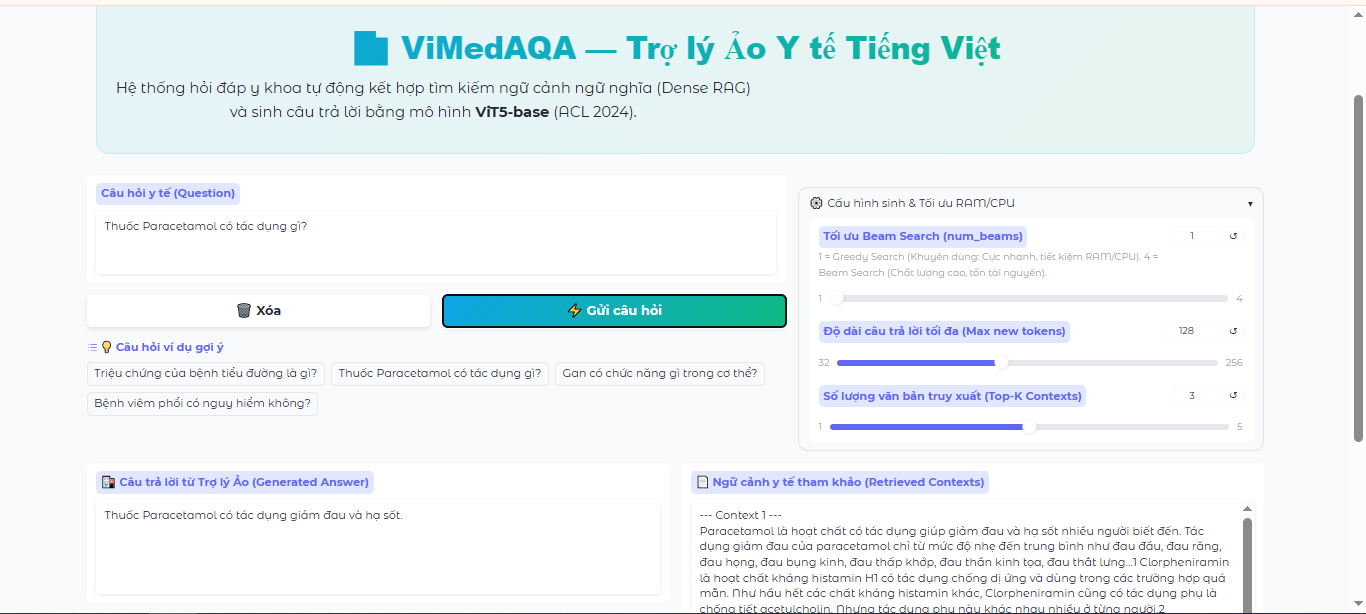
\includegraphics[width=0.85\textwidth]{figures/gradio_ui.png}
    \caption{Giao diện ứng dụng trợ lý ảo y tế ViMedAQA chạy thực tế trên HuggingFace Spaces}
    \label{fig:gradio_ui}
\end{figure}

Giao diện được tùy biến thiết kế (Custom CSS) với gam màu chủ đạo xanh ngọc và lục bảo (\texttt{linear-gradient(135deg, \#0ea5e9, \#10b981)}) mang lại cảm giác chuyên nghiệp, premium và tin cậy cho miền y tế. Người dùng có thể nhập câu hỏi tự nhiên ở khung bên trái, tinh chỉnh các thanh trượt cấu hình sinh (như số lượng chùm Beam Search $num\_beams$, số lượng ngữ cảnh truy xuất $top\_k$, và độ dài tối đa $max\_new\_tokens$). Khung bên phải sẽ hiển thị đồng thời hai kết quả trực quan: câu trả lời mạch lạc được sinh ra từ mô hình ViT5 và danh sách các văn bản ngữ cảnh y khoa tham khảo tương ứng được truy xuất từ FAISS để người dùng đối chiếu độ chính xác.

Ứng dụng demo được triển khai trực tuyến trên máy chủ đám mây của HuggingFace Spaces, phục vụ cộng đồng trải nghiệm thực tế tại địa chỉ:
\begin{itemize}
    \item \textbf{Liên kết ứng dụng Web Demo (HuggingFace Spaces):} \href{https://huggingface.co/spaces/kimquoc/vimedaqa-medical-qa}{kimquoc/vimedaqa-medical-qa}.
\end{itemize}
\chapter{Kết luận và hướng phát triển}
\section{Kết luận}
Đề tài đã hoàn thành xuất sắc mục tiêu xây dựng một hệ thống hỏi đáp tự động y khoa trừu tượng tiếng Việt chất lượng cao trên bộ dữ liệu ViMedAQA \cite{tran2024vimedaqa}. Thông qua một quy trình nghiên cứu chuẩn hóa và đồng bộ gồm tám phase (từ EDA dữ liệu, xây dựng baseline, fine-tuning mô hình sinh chuỗi, đến đóng gói công bố và triển khai ứng dụng), chúng tôi đã chứng minh năng lực thực tiễn vượt trội của các mô hình ngôn ngữ nhỏ (SLMs) chuyên biệt tiếng Việt khi được huấn luyện nội miền.

Hai mô hình chính là \textbf{ViT5-base} và \textbf{BARTpho-word} sau khi tinh chỉnh đều đạt hiệu năng rất cao, tiệm cận và thậm chí vượt qua siêu mô hình thương mại Llama-3.3-70B zero-shot ở một số chỉ số sinh chuỗi cụ thể. Đặc biệt, ViT5-base đạt điểm cân bằng lý tưởng trên cả độ đo trùng khớp từ ngữ bề mặt (BLEU-4 đạt \textbf{0,5005}, ROUGE-L đạt \textbf{0,6680}) và độ tương đồng ngữ nghĩa ngữ cảnh (BERTScore F1 đạt \textbf{0,8752}). Nghiên cứu cũng đã vạch rõ những đặc thù kỹ thuật của tokenizer và các giới hạn cố hữu của hệ đo lường tự động truyền thống đối với tiếng Việt chuyên ngành, đồng thời phát hiện và phân loại chi tiết ba failure modes y khoa phổ biến là lỗi lặp từ vô hạn, lỗi ảo tưởng thông tin và lỗi chi tiết quá mức. 

Cuối cùng, hệ thống đã được tích hợp thành công vào cấu trúc Dense RAG (kết hợp Bi-Encoder nhúng ngữ nghĩa và lập chỉ mục không gian vector FAISS tốc độ cao) và triển khai dưới dạng ứng dụng tương tác Gradio trực quan trên HuggingFace Spaces, tạo ra một sản phẩm hoàn thiện, có giá trị ứng dụng thực tiễn lớn trong việc hỗ trợ tra cứu thông tin y khoa ban đầu cho cộng đồng.

\section{Hướng phát triển trong tương lai}
Để nâng cao độ tin cậy và mở rộng quy mô ứng dụng của hệ thống, chúng tôi đề xuất ba định hướng nghiên cứu chuyên sâu tiếp theo:
\begin{enumerate}
    \item \textbf{Cơ chế RAG lai ghép (Hybrid Retrieval) và tối ưu hóa ngữ cảnh (Reranking):} Kết hợp sức mạnh bổ trợ lẫn nhau của cơ chế truy xuất thưa (BM25Okapi) và truy xuất dày đặc (Dense Bi-Encoder). Đồng thời, tích hợp mô hình đánh giá lại độ tương quan (Cross-Encoder Reranker) để chọn lọc và sắp xếp thứ tự ngữ cảnh y học chính xác nhất, giảm thiểu tối đa tạp âm và thông tin dư thừa đưa vào bộ sinh.
    \item \textbf{Đánh giá an toàn y khoa và giảm thiểu ảo tưởng triệt để (Fact-checking \& Medical Alignment):} Xây dựng cấu phần hậu xử lý tự động kiểm chứng nguồn thông tin y học sinh ra đối chiếu trực tiếp với ngữ cảnh gốc để phát hiện và ngăn chặn kịp thời các thông tin ảo tưởng y học nguy hiểm. Áp dụng kỹ thuật tối ưu hóa dựa trên phản hồi của chuyên gia y tế (RLHF - Reinforcement Learning from Human Feedback) để tinh chỉnh hành vi của mô hình tiệm cận với đạo đức và quy chuẩn lâm sàng.
    \item \textbf{Mở rộng dữ liệu đa chủ đề và tích hợp mô hình ngôn ngữ lớn nội địa:} Thu thập thêm dữ liệu chuyên sâu cho các chuyên khoa khó (như nhãn chủ đề y khoa Topic 1) và tiếp tục thực nghiệm tinh chỉnh trên các mô hình ngôn ngữ lớn mã nguồn mở có tri thức tiếng Việt mạnh mẽ hơn (như PhoGPT hoặc Vistral) nhằm tăng cường năng lực suy luận y học đa bước phức tạp.
\end{enumerate}

\clearpage
\bibliographystyle{ieeetr}
\bibliography{references}

\end{document}